\documentclass{sig-alternate}
%\documentclass{vldb}
%\documentstyle{article}
%\documentstyle[amsmath,amsthm,amssymb,twocolumn]{article}
%\usepackage{times}



\usepackage{MnSymbol} 
%\usepackage{MinionPro}
%\usepackage[mathlf,textlf,minionint]{MinionPro}
%\usepackage[T1]{fontenc}
%\usepackage{textcomp}
\usepackage{multirow}
%\usepackage{times}
\usepackage{pgfplots}
\usepackage{subfigure}
%\usepackage{amsmath,amssymb}
\usepackage{graphicx,color}
%\usepackage{verbatim}
%\usepackage{framed}
%\usepackage[ruled,vlined]{algorithm2e}

\usepackage[font={scriptsize,it}]{caption}


\begin{document}



%\newcommand{\agp}[1]{\smallskip\noindent \textcolor{red}{\it $\Rightarrow$ Aditya: #1}}
%\newcommand{\alkis}[1]{\smallskip\noindent \textcolor{red}{\it $\Rightarrow$ Alkis: #1}}
\newcommand{\SeeDB}{{\sf SeeDB}}
\newcommand{\calQ}{\mathcal{Q}}
\newcommand{\calR}{\mathcal{R}}
\newcommand{\att}[1]{{\text{#1}}}

\newtheorem{definition}{Definition}[section]
\newtheorem{example}[definition]{Example}
\newtheorem{goal}{Goal}[section]
\renewcommand{\baselinestretch}{0.995}

%\DeclareMathOperator*{\argmax}{arg\!\max}




%\newcommand{\histvis}{\mbox{\sc HistVis}}
\newcommand{\squishlist}{
   \begin{list}{$\bullet$}
    { \setlength{\itemsep}{0pt}
      \setlength{\parsep}{2pt}
      \setlength{\topsep}{0pt}
      \setlength{\partopsep}{0pt}
      \leftmargin=25pt
\rightmargin=0pt
\labelsep=5pt
\labelwidth=10pt
\itemindent=0pt
\listparindent=0pt
\itemsep=\parsep
    }
}
\newcommand{\squishend}{\end{list}}

\newenvironment{denselist}{
    \begin{list}{\tiny{$\bullet$}}%
    {\setlength{\itemsep}{0ex} \setlength{\topsep}{0ex}
    \setlength{\parsep}{0pt} \setlength{\itemindent}{0pt}
    \setlength{\leftmargin}{0.5em}
    \setlength{\partopsep}{0pt}}}%
    {\end{list}}

\newcommand{\eat}[1]{}
\newcommand{\papertext}[1]{#1}
\newcommand{\techreport}[1]{}

\newcommand{\techreporttext}[1]{}
\newcommand{\stitle}[1]{\vspace{0.25em}\noindent\textbf{#1}}




\title{SeeDB: Visualizing Database Queries Efficiently\vspace{-5pt}}
%\subtitle{\vspace{-10pt}[Vision Paper]\vspace{5pt}}



\numberofauthors{3}
\author{
\alignauthor
Aditya Parameswaran \\ 
\affaddr{Stanford University \& UIUC} \\
\affaddr{adityagp@illinois.edu} 
\alignauthor Neoklis Polyzotis \\ 
\affaddr{Google \& UCSC} \\ 
\affaddr{alkis@cs.ucsc.edu} 
\alignauthor Hector Garcia-Molina \\ 
\affaddr{Stanford University} \\ 
\affaddr{hector@cs.stanford.edu} 
}

\maketitle                                          

\vspace{-10pt}                                                     
                                             

\begin{abstract}
Data scientists rely on visualizations to interpret the data returned by queries, but finding the right visualization remains a manual task that is often laborious. We propose a DBMS that partially automates the task of finding the right visualizations for a query. In a nutshell, given an input query Q, the new DBMS optimizer will explore not only the space of physical plans for Q, but also the space of possible visualizations for the results of Q. The output will comprise a recommendation of potentially ``interesting'' or ``useful'' visualizations, where each visualization is coupled with a suitable query execution plan. We discuss the technical challenges in building this system and outline an agenda for future research.
\end{abstract}


\section{Introduction}\label{sec:intro}
\vspace{-10pt}
\begin{quote} {\em
... today's researchers must consume ever higher volumes 
of numbers that gush, as if from a fire hose ... 
}
\end{quote}
\vspace{-7 pt}
\noindent \hspace{80pt} --- R.M. Friedhoff and T. Kiely
\smallskip

Data analysts must sift through huge volumes of data
looking for valuable data-specific insights, trends, or anomalies.
This process involves selecting the ``right'' subset of the data,
and the ``right'' way to view it, so that the ``insights'' become apparent.
Moreover, the process is often ad-hoc and consumes a lot of the analyst's time.
Our vision is that {\em some especially cumbersome aspects} of this search 
for interesting insights can be automated.

To illustrate, consider the following interactive exploration workflow,
which we believe is often used in practice.

\noindent 
{\em Step (1):} First, the analyst poses a relational query 
to extract some subset of data they are interested in exploring.
For example, the analyst may select all records associated with
``stapler'' products.





\noindent {\em Step (2):} Then, the analyst considers several candidate views 
over this subset of data, formed by, say, aggregation and grouping;
the analyst must study all of these views one by one.
For example, one view may be total stapler sales by year,
while another view may be the quantity in stock by sales region.
Since these views have two-attributes each, we can view them
as 2-dimensional graphs. 
For example, Figure 1(a) may be the stapler sales (y-axis) by year (x-axis),
while Figure 1(c) may be the quantity (y-axis) by region (x-axis).
(Figures 1(b) and 1(d) are discussed below.)




\noindent {\em Step (3):} Next, the analyst steps 
through each view, and decides which views are ``interesting.''
This of course is the critical and time-consu\-ming step.
What makes a view like Figure 1(a) interesting or not?
Well, it all depends on the application semantics
and what we are comparing against.
For example, Figure 1(a) shows decreasing sales over time.
If we are in a recession and all product sales are down then this observation
is not very interesting. However, say that Figure 1(b) shows
the aggregate (all) product sales over the same time periods.
Then the stapler sales view goes against the general trend: 
overall sales are up, but stapler sales are going down.
In this case, the view is {\em potentially} ``interesting''
because it depicts a trend in the subset of data
that the analyst is interested in (i.e., stapler-related data)
that {\em deviates} from the trend in the overall data.
Of course, the analyst must decide if this deviation 
is truly an insight for this application.
Even so, our key insight is that we may be able to 
{\em identify and highlight to the analyst potentially interesting views 
using automated mechanisms based on deviation}.
By doing so, we eliminate the laborious process
of stepping through all possible views that the analyst currently 
performs.
Once we recommend potentially interesting views, we can let the analyst
make the final decision.

\pgfmathdeclarefunction{gauss}{2}{%
  \pgfmathparse{1/(#2*sqrt(2*pi))*exp(-((x-#1)^2)/(2*#2^2))}%
}

\pgfplotsset{ticks=none}

\begin{figure}[htp]
  \centering
  \vspace{-10pt}
    \subfigure[]
    {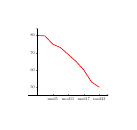
\begin{tikzpicture}[scale = 0.15]
      \begin{axis}[
      axis lines=center,
      axis on top=true,
      enlargelimits=0.15,
      symbolic x coords={mod2,mod3,mod5,mod7,mod11,mod13,mod17,mod19,mod23},
      ]
    \addplot[draw=red, ultra thick] coordinates 
      { (mod2,80) (mod3,79.7961) (mod5,75)
        (mod7,73) (mod11,69) (mod13,65)
        (mod17,60) (mod19,53) (mod23,50)};
    \end{axis}
    \end{tikzpicture}}
    \subfigure[]
    {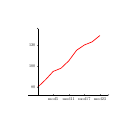
\begin{tikzpicture}[scale = 0.15]
    %   \begin{axis}[
    %   xmin=0, xmax=1.5,
    %   ymin=0, ymax=1.5,
    %   axis lines=center,
    %   axis on top=true,
    %   domain=0:1,
    %   ]
    % \addplot [mark=none,draw=red,ultra thick] {x};
    \begin{axis}[
      axis lines=center,
      axis on top=true,
      enlargelimits=0.15,
      symbolic x coords={mod2,mod3,mod5,mod7,mod11,mod13,mod17,mod19,mod23},
      ]
    \addplot[draw=red, ultra thick] coordinates 
      { (mod2,80) (mod3,87) (mod5,95)
        (mod7,98) (mod11,105) (mod13,115)
        (mod17,120) (mod19,123) (mod23,129)};
    \end{axis}
    \end{tikzpicture}}
    \subfigure[]
    {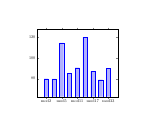
\begin{tikzpicture}[scale = 0.15]
%       \begin{axis}[every axis plot post/.append style={
%   mark=none,domain=-2:3,samples=50,smooth}, % All plots: from -2:2, 50 samples, smooth, no marks
%   axis x line*=bottom, % no box around the plot, only x and y axis
%   axis y line*=left, % the * suppresses the arrow tips
%   enlargelimits=upper] % extend the axes a bit to the right and top
%   \addplot {gauss(0,0.25)};
% \end{axis}
    \begin{axis}[
      ymin=70, ymax=120,
      axis on top =true,
      ybar,
      enlargelimits=0.15,
      symbolic x coords={mod2,mod3,mod5,mod7,mod11,mod13,mod17,mod19,mod23},
      ]
    \addplot coordinates 
      { (mod2,80) (mod3,79.7961) (mod5,114.4597)
        (mod7,85) (mod11,90.5600) (mod13,120)
        (mod17,87) (mod19,79) (mod23,90)};
    \end{axis}
    \end{tikzpicture}
    }
    \subfigure[]
    {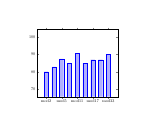
\begin{tikzpicture}[scale = 0.15]
      \begin{axis}[
      ybar,
      ymin=70, ymax=100,
      enlargelimits=0.15,
      symbolic x coords={mod2,mod3,mod5,mod7,mod11,mod13,mod17,mod19,mod23},
      ]
    \addplot coordinates 
      { (mod2,80) (mod3,82.7961) (mod5,87.4597)
        (mod7,85) (mod11,90.5600) (mod13,85)
        (mod17,87) (mod19,87) (mod23,90)};
    \end{axis}
    \end{tikzpicture}
    }
    \vspace{-13pt}
    \caption{Views (a), (b): Sales over Time. (c), (d): Quantity by Region.}\label{fig:plots}
    \vspace{-12pt}
 \end{figure}

Figures 1(c) and 1(d) illustrate a different type of deviation.
The first figure shows the distribution of staplers
across regions, while the second figure shows the
overall product distribution.
Again, the stapler view does not follow the general trend:
the regions that have the most staplers are not the larger regions
that have most product in stock.
The analysis must decide if this observation is interesting:
perhaps the region that has many staplers is near
the world-famous stapler-gun-wrestling contest,
in which case the observation is expected.
But perhaps there is a problem with the product shipping strategy,
in which case the deviation is very important.
% In this example as well, there is a deviation between
% the distribution in the subset of data that the analyst is interested in,
% and the rest of the data in the database.
% Thus, our goal is to automate the search for views that are {\em potentially}
% interesting, and to then let the analyst make the final decision.









\begin{figure}[t!]
\vspace{-15pt}
\begin{center}
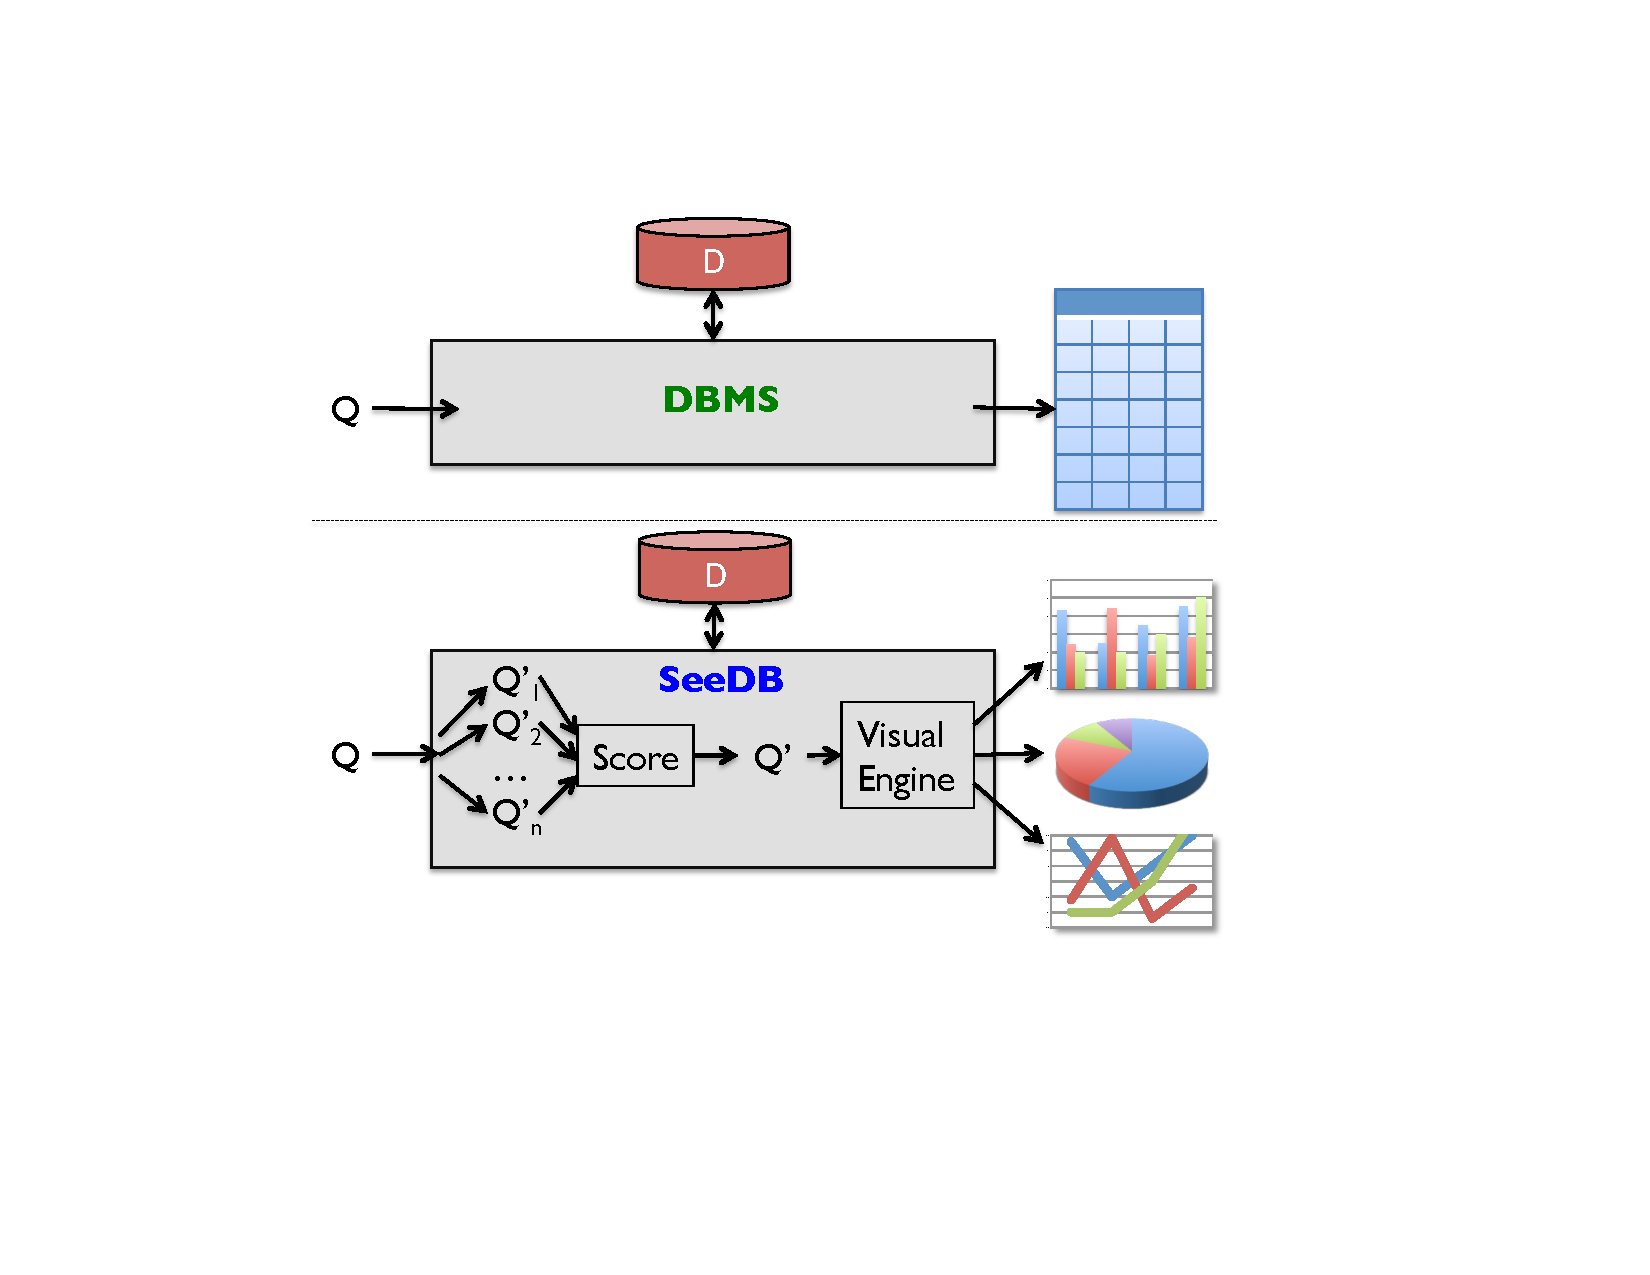
\epsfig{file=Images/comparison-diagram.pdf, width=1.5in, trim=3in 2.5in 3in 1in}
\end{center}
\vspace{-10pt}
\caption{\SeeDB\ Comparison with regular DBMS\label{fig:comparison} (The workflow for \SeeDB\ is only conceptual and need not happen in that order.)}
\vspace{-15pt}
\end{figure}

In this vision paper, we sketch our design for a new data base management system
(DBMS), \SeeDB, that automates the especially laborious 
aspects of the search for useful data insights.
Figure 2 depicts \SeeDB, together with a conventional DBMS.
In the conventional system, the user or analyst submits a query $Q$
and obtains data subsets.
Thus, conventional systems do not provide any means for the analyst 
to get intuitive visual insights directly.
In \SeeDB, the analyst also submits a query, but instead
automatically obtains views (or visualizations) of the query result
that are potentially of interest.
As illustrated in our examples,
these visualizations help the
analyst quickly interpret and understand specific
``interesting/useful'' aspects of the query result.
Thus, with \SeeDB, we fundamentally modify the
query-result paradigm of databases: \SeeDB\ is provided a query $Q$,
and outputs visualizations of interesting aspects
of $Q$.

Given a database and a query $Q$, \SeeDB\ considers a space of views 
$Q_1', \ldots, Q_n'$ that
are generated by adding to $Q$ additional relational operators, 
such that the results can be readily visualized 
(via the visual engine, depicted in Figure~\ref{fig:comparison}).
For instance, one possibility in our Staplers example was to 
add a group by and an aggregation giving a view corresponding to total sales of Staplers per region. 
We call these views $Q_1', \ldots, Q_n'$ the {\em discriminating views}.
To decide if a discriminating view is interesting, \SeeDB\ compares it
to the equivalent view obtained from the full database, using the
same operators.
For comparing the two views, \SeeDB\ 
uses a set of functions that captures how much the first view {\em deviates}
from the second.  
Prior work in the visualization community has identified
several functions for this purpose; however an important
issue is the feasibility of computing such functions on 
large databases.
These functions capture the deviations illustrated in
our initial example (e.g., different slopes), and draw
from existing functions that compare value distributions
(e.g., earth movers function).
Of course, \SeeDB\ is not tied to any particular function(s),
and allows the analyst to override the defaults using 
their own functions.
We say that \SeeDB\ computes the {\em utility} of discriminating 
view when it compares the discriminating view against the same
view on the database.

\techreport{Even if \SeeDB\ limits the discriminating views considered, the cost of computing utilities may be prohibitive. Thus, we will also suggest techniques for improving performance. For example, it may be possible to reuse some of the computations from evaluating one view, in evaluating the utility of another view. A different avenue for improving performance, is to provide approximate results, either by reducing the size of a view, or by computing its utility approximately.}



% Since the space of possible views that \SeeDB must explore is huge,
% for tractability the space must be constrained.
% Here we will suggest the following constraints,
% which we believe can be relaxed in the future.
% We focus on a database with a traditional star schema,
% and a query $Q$ on the fact table.
% (We illustrate these terms, as well as other terms 
% in this paragraph, in the example below.)
% \SeeDB considers 2-attribute views that are generated by adding to $Q$
% a single aggregation and group-by operator.
% We call these views the {\em discriminating views}.
% To decide if discriminating view $V$ is interesting, \SeeDB compares it
% to the equivalent view $V_D$ obtained from the full database, using the
% same aggregation and group-by operator.
% To determine if $V$ and $V_D$ are significantly different, \SeeDB uses
% a set of analyst-provided comparison functions.
% These functions capture the differences illustrated in
% our initial example (e.g., different slopes), and draw
% from existing functions that compare value distributions
% (e.g., earth movers function).
% We say that \SeeDB computes the {\em utility} of $V$
% when it compares it against $V_D$.

% Even if \SeeDB limits the discriminating views considered,
% the cost of computing utilities may be prohibitive.
% Thus, we will also suggest techniques for improving 
% performance. For example, it may be possible to reuse some of the
% computations from evaluating one view, in evaluating the utility of another view.
% A different avenue for improving performance, is to
% provide approximate results, either by reducing the size of a view,
% or by computing its utility approximately.

Our next example is a more detailed version of the previous example,
and clarifies the terms introduced.

\begin{example}\label{example}
\vspace{-10pt}
We focus on a database with a traditional star sch\-ema.
We operate on a single fact table $D$, containing information
about sales. The schema of $D$ comprises three dimension
attributes: \att{Product}, \att{Location}, and \att{Year}, and
one measure attribute: \att{Sales}.

Let us assume our analyst has entered a query with a
single selection predicate:
$Q \equiv \sigma_{(\att{Product = Staplers})}$.
The result contains too many tuples to examine individually, and
hence the analyst has to rely on some appropriate visualization in order
to glean interesting insights about the overall query result.

\SeeDB\ searches over all possible discriminating views that
can be obtained by adding a single aggregate and group by operator.
We initially focus on these two-attribute discriminating views
because they are easy to visualize using histograms or line plots.
(\SeeDB\ also considers more general views.)
One of these queries is 
$Q_1' = R_1(Q)$ where $R_1 \equiv \gamma_{\att{Location, sum(Sales)}}$.
This query tracks the sum of \att{Sales} over \att{Location}.
A possible result, $R_1(Q(D))$, is the discriminating view
shown in the top part of Table 2.
Another possible query is $Q_2' = R_2(Q)$, where $R_2 \equiv
\gamma_{\att{Year, sum(Sales)}}$, tracking the sum of
\att{Sales} over \att{Year}.
The bottom part of Table 2 shows a possible result of this
second view.


The next step is to score each view based on its utility, i.e., its
ability to show an interesting property of the query result. For this
purpose, \SeeDB\ obtains aggregate statistics for
\att{Sales} for \att{Location} and \att{Year} for the original full database.
(As we will see later, there
are interesting optimization opportunities if we can integrate this
step with the processing of $Q$.)
Table 1 shows the full database aggregates, i.e., $R_1(D)$ and $R_2(D)$
corresponding to our sample views.
(Note the missing $Q$.)
For the \att{Location} attribute, both $R_1(D)$ and $R_1(Q(D))$
have similar distributions.
(The fact that sales are uniformly lower in $R_1(Q(D))$ is not
surprising since $R_1(Q(D))$ only considers a fraction of the data.)
However, notice that the
distribution across \att{Year}s is very different for tuples
satisfying \att{Product = `Staplers'}. That is, demand for
\att{`Staplers'} seems to have not gone up, unlike the other products.
This unexpected behavior will be detected by \SeeDB\ when it
computes the utility of $R_2(Q)$, and hence $R_2(Q)$
(and not $R_1(Q)$) will be suggested to the analyst for further human evaluation.

\vspace{-10pt}
\end{example}


\begin{table}
{\scriptsize \center
\vspace{-10pt}
\begin{tabular}{|c|c|c|c|}
\hline
\multicolumn{4}{|c|}{\att{Location} Aggregates: $R_1(Q(D))$ } \\ \hline
Boston: 30 & Seattle: 40 & New York: 40
& San Francisco: 90  \\
\hline
 \hline 
\multicolumn{4}{|c|}{\att{Year} Aggregates: $R_2(Q(D))$} \\ \hline
2009: 50 & 2010: 40 & 2011: 60 & 2012: 50  \\
\hline
\end{tabular} 

\vspace{-10pt}
\caption{Aggregates for \att{Product = `Staplers'} \label{tab:new-agg}}
}
\end{table}


\begin{table}
\vspace{-10pt}
{\scriptsize \center

\begin{tabular}{|c|c|c|c|}
\hline
\multicolumn{4}{|c|}{\att{Location} Aggregates: $R_1(D)$} \\ \hline
Boston: 300 & Seattle: 300 & New York: 300
& San Francisco: 700  \\
\hline
 \hline 
\multicolumn{4}{|c|}{\att{Year} Aggregates: $R_2(D)$ } \\ \hline
2009: 100 & 2010: 200 & 2011: 500 & 2012: 800  \\
\hline
\end{tabular} 

\vspace{-10pt}
\caption{Original Aggregates\label{tab:original-agg}}
}
\vspace{-18pt}
\end{table}

\noindent Thus, there are several technical challenges that need to be addressed:

\begin{denselist}

\item For a given query, $n$, the total number of discriminating views, is likely to be very large to explore exhaustively and precisely. Even if we restrict ourselves to views that append a group-by and an aggregation, the number of choices depends on the number of aggregation methods and group-by attributes. Generating each of $R_1(Q(D)),$  $\ldots,$ $R_n(Q(D))$, scoring them on utility, and then picking the best one is certainly not feasible for most databases. Thus, we need mechanisms to prune the space of views and compute their utility approximately. This approach is reminiscent of how a query optimizer costs and prunes candidate execution plans, except that the objectives are different and hence may require different cost models and data statistics. In addition, given that the end result is consumed by an analyst, it may be preferable to recommend a visualization with lower utility but also lower cost to generate. This option creates a bi-criterion optimization problem, where possible visualizations may trade off between utility and cost.

\item Generating and scoring the discriminating views $R_i(Q(D))$ one-by-one may miss interesting optimization opportunities: First, we may share computation between discriminating views.  For example,
the results of two views with different aggregates but the same group-by may be computed together in one query, followed by projecting out to reveal the two individual views.  Second, by evaluating the discriminating views in a deliberate order, we may be able to prune views with
low utility (without evaluation) that are definitely not going to be recommended to the analyst.

\item Since visualizations tend to convey approximate information, e.g., a trend in a line plot may be more important than knowing the exact coordinates of each point, we can introduce approximations as part of \SeeDB.  Thus, the utility of a discriminating view may be computed approximately but efficiently, and the recommended discriminating views can be populated with approximate results, based on synopses of the base data or of the query result, that can be generated much more efficiently.

\end{denselist}

\noindent Over the past few years, there has been a significant
effort from the visualization community to provide interactive tools
for data analysts. In particular, tools such as ShowMe, Polaris, and
Tableau~\cite{DBLP:journals/cacm/StolteTH08,
  DBLP:journals/tvcg/MackinlayHS07} provide a canvas for data analysts
to manipulate and view data, tools such as
Wrangler~\cite{DBLP:conf/chi/KandelPHH11} allow data analysts to
transform and clean data, and tools such as
Profiler~\cite{DBLP:conf/avi/KandelPPHH12} allow users to visualize
simple anomalies in data.  However, unlike \SeeDB, these tools have
little automation; in effect, it is up to the analyst to generate a
two-column result (like the result of the discriminating view)
to be visualized.

In this paper, we present our goals formally, and then present our initial design for \SeeDB, along with the underlying challenges.



% \section{Introduction}\label{sec:intro}
% \vspace{-10pt}
% \begin{quote} {\em
% ... today's researchers must consume ever higher volumes 
% of numbers that gush, as if from a fire hose ... 
% }
% \end{quote}
% \vspace{-3	pt}
% \noindent \hspace{80pt} --- R.M. Friedhoff and T. Kiely~\cite{friedhoff1990eye}
% \smallskip


% Data analysts now form an integral part of most organizations, 
% routinely exploring and analyzing automatically collected data, 
% to provide valuable data-specific insights. 
% Since database systems have several desirable properties, 
% including declarative query formulation and efficient processing 
% of large volumes of data, it is natural to consider database systems as a primary tool for supporting data analysts doing interactive data exploration. 
% Several data analysts do use database systems for this purpose, but the end-to-end task of interactive exploration remains cumbersome and in some cases unintuitive~\cite{DBLP:conf/sigmod/Hanrahan12, DBLP:journals/pvldb/HeerH09}.

% To illustrate, consider one such interactive exploration workflow involving 
% a database:

% \noindent 
% {\em Step 1:} First, the analyst may pose a relational query 
% to extract some subset of data they are interested in exploring. 


% \noindent {\em Step 2:} Then, the analyst considers several candidate views 
% over this subset of data, formed by, say, aggregation and grouping.
% For concreteness, we assume a single aggregation and group-by operator.
% Unlike the raw subset of data, 
% the results of these views can in fact be 
% visually depicted using line diagrams or
% histograms like the ones depicted below (a)---(d): here, even though
% the axes are not visible, the aggregated attribute is along the y-axis,
% and the group-by attribute is along the x-axis.

% \noindent {\em Step 3:} Next, the analyst then  
% visually compares the results of these views on the subset of data, 
% to the same views on the entire database, to find the views
% with the most ``utility''. 
% For instance, let (a) depict the visualization of one view 
% over the subset of data, and let (b) depict the visualization
% of the same view over the underlying database.
% Here, there is a clear deviation in the ``distribution'': 
% while the view on the subset shows the aggregate going down,
% the same view on the underlying database goes up.
% Thus, the view, being different on the subset of data
% from that on the complete database,
% may be interesting and useful to an analyst
% in that it depicts one aspect where the subset of data
% deviates from the complete database.
%  Similarly, between (c) and (d), once again, 
% there is a deviation in the distribution:
% the visualization of the view on the subset in (c) 
% has a much more narrower peak than
% the visualization in (d).

% Thus, overall, database systems do not provide any 
% means to explore or interpret a large query result except to output data for further processing.  How to process or visualize this output remains a challenging task that falls on the data analyst, who is now faced with yet another data analysis task, this time on the output of the query instead of the original database.




% \pgfmathdeclarefunction{gauss}{2}{%
%   \pgfmathparse{1/(#2*sqrt(2*pi))*exp(-((x-#1)^2)/(2*#2^2))}%
% }

% \pgfplotsset{ticks=none}


% \begin{figure}[htp]
%   \begin{center}
% \vspace{-10pt}
%     \subfigure[]
%     {\begin{tikzpicture}[scale = 0.2]
%       \begin{axis}[
%       xmin=0, xmax=1.5,
%       ymin=0, ymax=1.5,
%       axis lines=center,
%       axis on top=true,
%       domain=0:1,
%       ]
%     \addplot[mark=none,draw=red,ultra thick] {1-x};
%     \end{axis}
%     \end{tikzpicture}}
%     \subfigure[]
%     {\begin{tikzpicture}[scale = 0.2]
%       \begin{axis}[
%       xmin=0, xmax=1.5,
%       ymin=0, ymax=1.5,
%       axis lines=center,
%       axis on top=true,
%       domain=0:1,
%       ]
%     \addplot[mark=none,draw=red,ultra thick] {x};
%     \end{axis}
%     \end{tikzpicture}}
%     \subfigure[]
%     {\begin{tikzpicture}[scale = 0.2]
%       \begin{axis}[every axis plot post/.append style={
%   mark=none,domain=-2:3,samples=50,smooth}, % All plots: from -2:2, 50 samples, smooth, no marks
%   axis x line*=bottom, % no box around the plot, only x and y axis
%   axis y line*=left, % the * suppresses the arrow tips
%   enlargelimits=upper] % extend the axes a bit to the right and top
%   \addplot {gauss(0,0.25)};
% %  \addplot {gauss(1,0.75)};
% \end{axis}
%     \end{tikzpicture}
%     }
%     \subfigure[]
%     {\begin{tikzpicture}[scale = 0.2]
%       \begin{axis}[every axis plot post/.append style={
%   mark=none,domain=-2:3,samples=50,smooth}, % All plots: from -2:2, 50 samples, smooth, no marks
%   axis x line*=bottom, % no box around the plot, only x and y axis
%   axis y line*=left, % the * suppresses the arrow tips
%   enlargelimits=upper] % extend the axes a bit to the right and top
%  % \addplot {gauss(0,0.5)};
%   \addplot {gauss(1,0.85)};
% \end{axis}
%     \end{tikzpicture}
%     }
%   \end{center}
%   \vspace{-25pt}
%  \end{figure}







% \begin{figure}[t!]
% \vspace{-10pt}
% \begin{center}
% 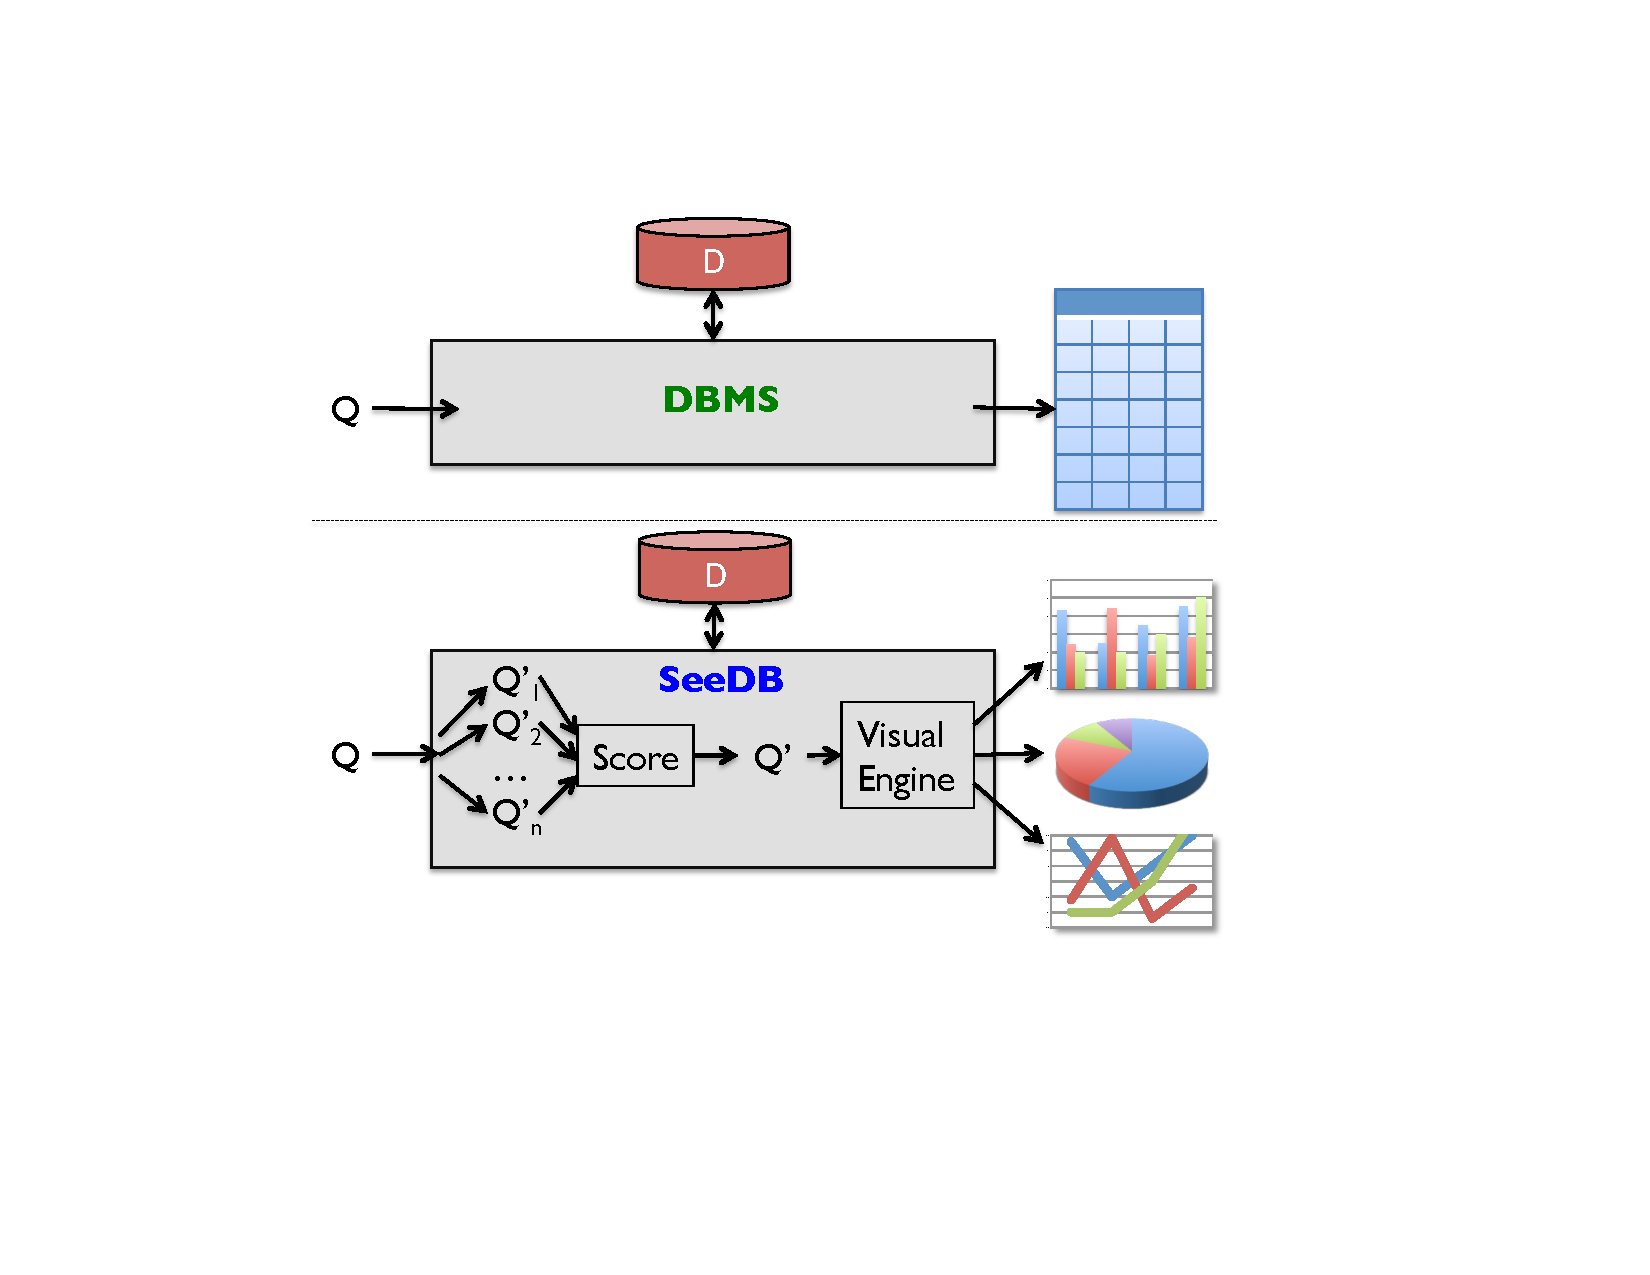
\epsfig{file=Images/comparison-diagram.pdf, width=2in, trim=3in 2.5in 3in 1in}
% \end{center}
% \caption{\SeeDB\ Comparison with regular DBMS\label{fig:comparison} (The workflow for \SeeDB\ is only conceptual and need not happen in that order.)}
% \vspace{-10pt}
% \end{figure}

% In this vision paper, we present a new data base management system (DBMS), \SeeDB, by promoting the notion of visualization 
% to a first class citizen inside the DBMS.
% A conceptual workflow for \SeeDB\ is depicted alongside the traditional DBMS workflow in Figure~\ref{fig:comparison}. As depicted, \SeeDB\ takes as input a query $Q$, just like in a traditional database system, but presents the data analyst with visualizations of the query result on the database $D$, instead of the raw tuples in the query result. 
% Like in our workflow described earlier, these visualizations help the data analyst to quickly interpret and understand specific ``interesting/useful'' aspects of the query result. In addition, these visualizations come ``without any effort'', i.e., the analyst does not have to do any additional work to generate them. 

% As a first step in selecting a good visualization, \SeeDB\ identifies a space of possible visualizations for $Q$. 
% Each visualization stems 
% from what we term as a {\em discriminating view}.
% Discriminating views are simple transformations of $Q$ to 
% $Q_1' = R_1(Q), Q_2' = R_2(Q), \ldots, Q_n' = R_n(Q)$ ---
% crafted by appending additional relational operators to $Q$.
% After generating an interesting set of discriminating views, 
% \SeeDB\ will score them according to their utility, and select
% one (or several) that will be recommended to the analyst.  
% The visual engine in \SeeDB\ (see Figure~\ref{fig:comparison}) 
% uses standard rules of thumb~\cite{DBLP:journals/cacm/StolteTH08, DBLP:journals/tvcg/MackinlayHS07,DBLP:conf/avi/KandelPPHH12} to dictate which graphical layout (histogram, bar chart, line diagram, etc.) would be the most appropriate to depict the result of each of the recommended discriminating views.

% We now present an example to help clarify this workflow:

% \begin{example}\label{example}
% In this example we operate on a single table, containing information about sales. The schema of the table comprises three dimension attributes, namely, \att{Product}, \att{Location}, and \att{Year}, and a single measure attribute \att{Sales}. 

% Let us assume our user has entered a simple query that consists of a single selection predicate: $Q \equiv \sigma_{(\att{Product = Staplers})}$. Following a typical use case in practice, we assume that the result contains too many tuples to examine individually, and hence the user has to rely on some appropriate visualization in order to glean interesting insights about the overall query result. 
 
% In our simple example, we assume that there are two such discriminating views, termed $R_1(Q)$ and $R_2(Q)$, where $R_1 \equiv \gamma_{\att{Location, sum(Sales)}}$ and $R_2 \equiv \gamma_{\att{Year, sum(Sales)}}$. In this setup, $R_1$ tracks the sum of \att{Sales} over \att{Location}, whereas $R_2$ tracks the sum of \att{Sales} over \att{Year}. 
% Note that these discriminating views correspond to appending a group-by and an aggregation over $Q$. Later, we identify this specific class of discriminating views as an important special case for \SeeDB, since the result of these views corresponds to two-column tables that can be directly visualized using standard techniques such as histograms or line plots. Of course, our plan is to consider more general classes of discriminating views that correspond to richer visualizations, e.g., multi-column tables that can be visualized as stacked bar-charts. 
% Overall, even in the special case of discriminating views based on group-by and aggregations, there is a large space of discriminating views to consider, and managing (and most importantly pruning) this space is one of the technical challenges we have to tackle.

% The next step is to score each view based on its utility, i.e., its ability to show an interesting property of the query result. For this purpose, let's say that \SeeDB\ obtains aggregate statistics for \att{Sales} for \att{Location} and \att{Year} by processing both the original database and the results of $Q$. As we will see later, there are interesting optimization opportunities if we can integrate this step with the processing of $Q$. Tables~\ref{tab:original-agg} and~\ref{tab:new-agg} show these statistics for the original database and the results of $Q$, respectively. Unlike \att{Location}, which seems to have a similar distribution for both the original table as well as the tuples that satisfy \att{Product =} \att{`Staplers'}, the distribution across \att{Year}s is very different for tuples satisfying \att{Product = `Staplers'}. That is, demand for \att{`Staplers'} seems to have not gone up, unlike the other products. Thus, \SeeDB\ can recommend $R_1(Q)$ as a useful visualization for $Q$ (e.g., in the form of a bar chart or a line plot), since it seems to convey some useful intuition for the result of $Q$. 

% \end{example}

% \begin{table}
% \vspace{-10pt}
% {\small \center

% \begin{tabular}{|c|c|c|c|}
% \hline
% \multicolumn{4}{|c|}{\att{Location} Aggregates} \\ \hline
% Boston: 300 & Seattle: 300 & New York: 300
% & San Francisco: 700  \\
% \hline
%  \hline 
% \multicolumn{4}{|c|}{\att{Year} Aggregates} \\ \hline
% 2009: 100 & 2010: 200 & 2011: 500 & 2012: 800  \\
% \hline
% \end{tabular} 

% \vspace{-10pt}
% \caption{Original Aggregates\label{tab:original-agg}}
% }
% \end{table}

% \begin{table}
% {\small \center

% \begin{tabular}{|c|c|c|c|}
% \hline
% \multicolumn{4}{|c|}{\att{Location} Aggregates} \\ \hline
% Boston: 30 & Seattle: 40 & New York: 40
% & San Francisco: 90  \\
% \hline
%  \hline 
% \multicolumn{4}{|c|}{\att{Year} Aggregates} \\ \hline
% 2009: 50 & 2010: 40 & 2011: 60 & 2012: 50  \\
% \hline
% \end{tabular} 

% \vspace{-10pt}
% \caption{Aggregates for \att{Product = `Staplers'} \label{tab:new-agg}}
% }
% \vspace{-10pt}
% \end{table}


% \noindent Thus, there are several technical challenges that we have to solve in implementing \SeeDB:

% \begin{denselist}

% \item We need to define a scoring function that operationalizes the notion of utility for a discriminating view. Prior work in the visualization community provides some initial directions to tackle this challenge, but an important issue is the feasibility of computing such a function on large databases. 

% \item For a given query, $n$, the total number of discriminating views, is likely to be very large to explore exhaustively and precisely. Even if we restrict ourselves to discriminating views that append a group-by and an aggregation, the number of choices depends on the number of aggregation methods and the possible subsets of group-by attributes. Generating the results for $Q(D)$, then evaluating $Q_1'(D) = R_1(Q(D)),$ $Q_2'(D)=R_2(Q(D)),$ $\ldots, $ $Q_n'(D) = R_n(Q(D))$, scoring them, and then picking the best one is certainly not feasible for all but really small data bases. Thus, we need mechanisms to prune the space of views and compute their utility approximately. This approach is reminiscent of how a query optimizer costs and prunes candidate execution plans, except that the objective function is different and hence may require different cost models and different data statistics. In addition, given that the end result is consumed by an analyst interested in data exploration, it may be preferable to recommend a visualization that has lower utility but also lower cost to generate. This option creates a bi-criterion optimization problem, where possible visualizations may trade off between utility and cost.

% \item Generating and scoring the discriminating views $R_i(Q(D))$ one-by-one
% may miss interesting optimization opportunities: 
% First, we may share computation between discriminating views. 
% For example, the results of 
% two discriminating views dealing with different aggregates
% with the same group-by may be computed together in one query, 
% followed by projecting out to reveal the two individual views. 
% Second, by evaluating the discriminating views in a deliberate order,
% we may be able to prune discriminating views with low utility 
% (without evaluation)
% that are definitely not going to 
% contribute to the views recommended to the analyst.

% % \item Generating and scoring the discriminating views $R_i(Q(D))$ after $Q$ is evaluated may miss interesting optimization opportunities, e.g., using an index on the base data to compute a specific group-by. Thus, one approach would be to score discriminating views before $Q$ is evaluated and then create one unified execution plan for computing $Q$ and the views with the highest utility. On the other hand, waiting for $Q$ to be evaluated allows \SeeDB\ to inspect the result and thus evaluate better the utility of different discriminating views. One may also imagine a hybrid approach, where \SeeDB\ interleaves the evaluation of $Q$, the generation of discriminating views and the computation of their utility. Selecting the right strategy is a non-trivial optimization problem. 

% \item Since visualizations
% tend to convey approximate information themselves, e.g.,
% a trend in a line plot may be more important than knowing
% the exact coordinates of each point, we can introduce
% approximations as part of \SeeDB. 
% In this fashion, the utility of a discriminating view
% may be computed approximately but efficiently, 
% and the recommended discriminating views can be populated
% with approximate results, based on synopses of the base data
% or of the query result, that can be generated much more efficiently.


% % \item Taking into account the fact that visualizations tend to convey approximate information themselves, e.g., a trend in a line plot may be more important than knowing the exact coordinates of each point, we can introduce approximate query answering as a main component of \SeeDB. In this fashion, the recommended discriminating views can be populated with approximate results, based on synopses of the base data or of the query result, that can be generated much more efficiently. This option introduces an additional criterion in our optimization space thus leading to a three-way tradeoff among cost, utility, and approximation. An important challenge is quantifying the effect of approximation on the visualized data so that the data analyst can interpret the output of \SeeDB\ in a meaningful way.

% \end{denselist}

% \noindent Over the past several years, there has been a significant effort from the visualization community to provide interactive tools for data analysts. In particular, tools such as ShowMe, Polaris and Tableau~\cite{DBLP:journals/cacm/StolteTH08, DBLP:journals/tvcg/MackinlayHS07} provide a canvas for data analysts to manipulate and view data, tools such as Wrangler~\cite{DBLP:conf/chi/KandelPHH11} allow data analysts to transform data and cleanse it, and tools such as Profiler~\cite{DBLP:conf/avi/KandelPPHH12} allow users to identify simple anomalies in data. 
% However, unlike \SeeDB, these tools have little automation; in effect, it is up to the analyst to generate a two-column result (similar to the result of the discriminating view) to be visualized. 

% In this short paper, we present our goals formally, and then present a space of alternative choices for \SeeDB, along with the underlying technical challenges. 

\vspace{-3pt}
\section{System Objectives}

We now state the goals of \SeeDB\ more formally, 
to provide a blueprint for the system design sections that follow. 
When doing so, we deliberately focus on a simple setting to ground our discussion.
However, the setting we consider is an important use-case that occurs often
in practice, and was the focus of our illustrative example. 
We will consider advanced variants in Section~\ref{sec:extensions}.

\stitle{Concrete Goals:} We consider a database $D$ with a snowflake schema,
with dimension attributes $A$, measure attributes $M$, and potential aggregate
functions $F$ over the measure attributes.
We limit the class $\calQ$, of queries posed over $D$,  
to be those that select a horizontal fragment of the fact table. 
The selection of the fragment can be done with selection predicates
on the fact table, or on dimension tables through key/foreign-key joins. 
Intuitively, the idea is that the analyst specifies their interest 
in examining facts that satisfy specific conditions. 
\SeeDB\ will identify visualizations 
that show some interesting properties of these facts.

Given a query $Q$ in $\calQ$, we define $\calR_Q$,
the set of all discriminating views, to be
the set of views that perform a group-by and some aggregation 
over the results of $Q$. 
For simplicity, we assume that a discriminating view 
$R$ in $\calR_Q$ performs a group-by on a single attribute $a \in A$, 
and applies an aggregation function $f \in F$ 
on a single measure attribute $m \in M$. 
A view in this class corresponds to a two-column table 
that shows how the value of $f(m)$ varies with values of attribute $a$. 
This table can be directly visualized using a histogram, 
a bar chart or a line plot. (We consider generalizations in Section 4.)

We also assume the existence of a function $U(R)$ that can characterize the utility of each view $R(Q)$ in $\calR_Q$ (higher is better). For now, we focus on picking discriminating views that optimize $U(R)$ with latency as low as possible: we return to more general objectives in Section~\ref{sec:extensions}. Thus, our concrete goal is:
\vspace{-1pt}
\begin{goal}
\vspace{-3pt}
Given $Q \in \calQ$ and a positive integer $K$, find $K$ discriminating views $R_i \in \calR_Q$, such that the $R_i$ have the largest values of $U(R_i)$ among those in $\calR_Q$, and the total latency is minimized.
\vspace{-3pt}
\end{goal}
\vspace{-2pt}
\stitle{Operationalizing Utility:}
One of the key challenges behind \SeeDB\ 
is formalizing the utility function $U(R)$ for a discriminating view $R$. 
There are many choices for $U$ and we expect \SeeDB\ 
to recommend views that score high on several metrics. 
As discussed previously, the proposed metric tries to capture the idea of ``deviation'' between distributions, i.e., a view has high utility if its contents show a trend that deviates from the corresponding trend in the original database.  

We first define some notation. For any discriminating view $R_i$ 
in the class defined above, we note that $R_i(D)$ and $R_i(Q(D))$ 
are both two column tables. 
A two-column table can be represented using a weight vector.
We let the weight vector $W_{a, f(m)}$ represent the 
result of $R_i(D) = \gamma_{a, f(m)}(D)$, i.e., 
distribution of the aggregate function $f$ on the measure quantity $m$ 
across various values of the attribute $a$. Going back to our example, it follows that 
\vspace{-4pt}
\[
\vspace{-3pt}
W_{\att{Year, sum(Sales)}} = (2009: 100, 2010: 200, 2011: 500, 2012: 800)
\vspace{-2pt}
\]
\noindent Here $m$ is \att{Sales}, $f$ is the sum, and $a$ is the \att{Year} attribute. 
Then, we let $W_{a, f(m)}^Q$ represent the (changed) distribution of $R_i(Q(D))$, 
the aggregated quantity $m$ across values of the attribute $a$, 
when restricted to the result of the query $Q$. Thus,
\vspace{-5pt}
\[
\vspace{-3pt}
W_{\att{Year, sum(Sales)}}^{\sigma_{\att{Prod = `Staplers'}}} 
= (2009: 50, 2010: 40, 2011: 60, 2012: 50)
\vspace{-2pt}
\]

\noindent 
The utility $U$ of a discriminating view $\gamma_{a, f(m)}$ 
is defined to be the distance between $W_{a, f(m)}^Q$, and $W_{a, f(m)}$:
$U(\gamma_{a, f(m)}) = S(W_{a, f(m)}^Q, $ $W_{a, f(m)})$
where $S$ is a distance metric. 
The higher $S$ is, the more useful a discriminating view is. 
Common distance metrics used in visualization 
literature include K-L divergence~\cite{wikipedia-KL}, 
Jenson-Shannon distance~\cite{wikipedia-JS,entropy-vis}, 
and earth mover distance~\cite{wikipedia-prob-dist}. 
Wang~\cite{entropy-vis} provides a good overview 
of the metrics used in scientific visualizations, 
while \cite{wikipedia-prob-dist} provides a summary 
of probability-based distance metrics. 
As discussed earlier, we do not prescribe 
any specific distance metrics, 
instead, we plan to support a whole range of distance metrics, 
which can be overridden by the data analyst. 


\papertext{We show in our extended paper~\cite{tr} that in our example, we get the right discriminating view (i.e., that of \att{Year}) when we consider the metrics mentioned above: the utility for \att{Year} is significantly higher than that for \att{Location} for each of the metrics considered.}

\techreport{We now show for a couple of distance metrics, we get the right discriminating view (i.e., that of \att{Year}). The metric that is perhaps the easiest to explain is Earth Mover's Distance (EMD), used in many graphics visualization applications. Simply put, the metric measures how much probability ``earth'' would be necessary to transform one probability distribution into another. In our example, our normalized weight vectors for \att{Year} are (ignoring the \att{Year} field): $(0.06, $ $0.13,$ $0.31, $ $0.50)$ and $(0.25, 0.20,$ $ 0.30, 0.25)$. Here, the amount of ``earth'' that needs to be moved (and therefore $S$) is around 0.26. For \att{Location}, the normalized weight vectors are $(0.19, 0.19, 0.19, 0.43)$ and $(0.15,$ $0.2, 0.2, 0.45)$. Here, the amount of earth that needs to be moved is around $0.03$. Thus, \att{Year}, is a much more informative attribute to visualize.

We can also consider the Jenson-Shannon distance (a normalized version of the well-known Kullback-Liebler distance~\cite{wikipedia-KL}), used in many visualization applications, defined formally as (where $W_1, W_2$ are two normalized weight vectors): $$S(W_0, W_1) = H((W_0 + W_1)/2) - H(W_0)/2 - H(W_1)/2.$$ For \att{Year}, we have: $1.31 - (1.13/2 + 1.376/2) = 0.057$. For \att{Location}, we have: $1.300 - (1.309/2 + 1.287/2) = 0.002$. Thus, once again, \att{Year} is a much more informative attribute to visualize.}

\vspace{-5pt}
\section{Initial Design}
Our initial design for \SeeDB\ is as a simple wrapper over an existing database system. One straightforward workflow is as follows:
\begin{denselist}
\item {\em Step 1:} Enumerate all discriminating views $R \in \calR_Q$ and evaluate utility $U(R)$ (i.e., compute $W_{a, f(m)}^Q$ and $W_{a, f(m)}$) by issuing the corresponding counting queries to the DBMS. Select the $K$ views with highest $U(R)$. 
\item {\em Step 2:} Compute the results of these $K$ views using the DBMS, then forward the results to the visual engine.
\end{denselist}

\noindent 
It is clear that this workflow suffers from several inefficiencies. We now discuss potential optimizations, some of which require new query processing schemes specialized for the problem at hand.


\stitle{Approximate Utility Computation:} 
We can speed up Step 1 by computing the utilities of discriminating views approximately. Naturally, we would want the approximations to be accurate enough to select a good set of views for Step 2.
\techreport{In any case, \SeeDB\ should avoid selecting useless views in the output.} 

Sampling is one possible approximation method: We construct a sample of the query result $Q(D)$, 
and the underlying data $D$, and use these samples to compute approximate weight vectors $W_{a, f(m)}^Q$ and $W_{a, f(m)}$. (In fact, the latter, which does not depend on $Q$, can be computed before any queries are issued.) The question of how large a sample of $Q$ is necessary to enable the weight vectors $W_{a, f(m)}^Q$, for all $a, f, m$, to have high accuracy is, to the best of our knowledge, still open. Techniques from sampling for aggregation~\cite{DBLP:conf/vldb/Gibbons01}, and more generally, approximate query processing~\cite{wavelets, count-min-sketches} may be relevant here.

Ideally, we would want error bounds on the resulting approximate utilities, in order to enable \SeeDB\ to select views of provably high utility and avoid views of provably low utility. These guarantees may depend on the specific metric used. For instance, approximation guarantees on the magnitudes of the weight vectors may directly translate to guarantees on the earth mover distance (a simpler metric), but not the Jenson-Shannon distance (a complex metric).

\stitle{Searching the Space of Discriminating Views:} 
The space of discriminating views may be too large to search exhaustively in an efficient manner, particularly if \SeeDB\ relies on exact utility computation. Instead, it may be possible to prune the search space by leveraging relationships between discriminating views in terms of utility. For instance, functional dependencies among grouping attributes can help us infer that certain views will have the exact same utility by virtue of having the same groups. Furthermore, the search strategy that navigates the space of views may also take into account inter-dependencies: for instance,  investing computational resources to determine that a view has provably low utility would be useful, if this determination will lead to the pruning of several other views correlated with the specific view. 

%A related issue concerns the search strategy to navigate and prune the space of views. The strategy may take into account the specifics of the pruning rules mentioned above. For instance, it would be beneficial to invest computational resources in determining that a view has provably low utility if this will lead to the pruning of several other views whose utilities are correlated with the specific view. The search strategy can also leverage approximate utility computations in order to guide its choices. 

\stitle{Multi-Query Optimization:} 
Step 2 comprises the evaluation of $K$ queries and so raises opportunities for multi-query optimization~\cite{DBLP:journals/tods/Sellis88}. For instance, if we are recommending several discriminating views with the same group-by attribute, we may combine the computation of the views into a single group-by query with multiple aggregations (one per view). We expect that the opportunities to share computation will increase with more complex queries and views.   

Multi-query optimization may also be used to optimize utility computation (Step 1). For instance, multi-query optimization may reveal that $W_{a, f_i(m)}^Q$ may be computed together for all $i$. Additionally, since we make repeated calls to evaluate $W_{a, f(m)}^Q$ for different $a, f, m$, we can instead first materialize the query result $Q(D)$ and then compute the weight vectors $W_{a, f(m)}^Q$ by issuing queries on the materialized result. Materializing $Q(D)$ can also help in evaluating $R(Q(D))$ for each selected discriminating view $R$ in Step 2.

\stitle{Fusing the Two Steps:}
Up to this point we considered view selection and view computation as two separate stages inside \SeeDB. Alternatively, we may fuse the two stages in order to share work between the computation of utilities (Step 1) and the evaluation of view queries (Step 2), thus reducing end-to-end latency. 

Computing $U(R)$ requires knowledge about the contents of $R$, and therefore, we compute $U(R)$ and $R(Q(D))$ together. Since it may be prohibitively expensive to compute these quantities for each $R$, and since the end goal is to recommend only $K$ views, we may employ approximate utility computation coupled with a pruning rule. Specifically, suppose that is it possible to schedule the computation of $Q(D)$ and receive its output in a random order (e.g., as described in~\cite{dbo}). \SeeDB\ will then observe a sample of increasing size as it consumes the output of $Q(D)$. Processing the output involves two tasks: (a) updating a running estimate of the utility of each view (leveraging the fact that the observed output is a sample of $Q(D)$), and (b) updating the current contents of unpruned views using hash-based aggregation. \SeeDB\ can use the running utility estimates to prune views of low utility. Overall, as \SeeDB\ processes $Q(D)$ it can make progress towards both selecting the top-$K$ views and computing their contents. Thus, this specialized query-processing strategy can reduce \SeeDB's end-to-end latency but it comes with higher resource requirements (since many group-by queries need to be processed concurrently).


\techreport{However, processing many queries concurrently is essentially the same as multi-query optimization and so we expect it to have a similar resource footprint. Moreover, it is possible to partition the set of views and apply this strategy to select the top-$K$ views in each part, and subsequently select the final top-$K$ views in a post-processing step. Each part will involve fewer views and hence require fewer resources, but the total work to select the top-$K$ views will be higher. }

\eat{
\stitle{Statistics and Adaptation:} 
Even for a single input query $Q$, \SeeDB\ typically computes the results of many SQL queries using the DBMS --- both for computing utility of discriminating vies, and for computing the results of the selected discriminating views. It may be advantageous to compute the results of some queries in advance, in order to obtain better or more accurate distribution statistics on $D$, so that the remaining queries to the DBMS can benefit from better optimization based on accurate statistics.

For instance, the \SeeDB\ optimizer can choose to compute $Q(D)$ first, followed by estimating statistics, which may then be used to more efficiently compute the results of the discriminating views.Overall, there is an interesting space of possibilities that may also benefit from prior work on adaptive query optimization for conventional queries~\cite{DBLP:journals/ftdb/DeshpandeIR07}.
}

% The \SeeDB\ optimizer has three alternatives to choose from for 
% a given discriminating view $R_i(Q)$:
% First, it can chose to optimize and execute first the part 
% of the logical plan corresponding to $Q$, i.e., everything except $R_i$, 
% in order to materialize the query result. 
% Accurate distribution statistics of $Q(D)$ can then be used
% to better estimate the utility and latency of $R_i$, 
% which can be computed in a second phase.
% The downside, however, is that the optimizer may miss opportunities 
% to push down the $R_i$ operators inside the execution of $Q$. 
% A second method is to rely entirely on statistics on the base data,
% for both utility and latency computation, although
% estimation errors may affect the optimal choices for the discriminating view.
% A third method is a hybrid between the previous two,
% where some part of $Q$ is optimized and executed, and the intermediate 
% results materialized. 
% This can improve the accuracy of estimating the utility and latency metrics 
% while still maintaining the possibility of pushing down the $R_i$ operators. 
% Overall, there is an interesting space of possibilities that matches 
% previous works on query optimization for conventional queries\cite{DBLP:journals/ftdb/DeshpandeIR07}.


\vspace{-5pt}
\section{Enhancements and Extensions}\label{sec:extensions}

We now present some enhancements that may further improve the analyst's user experience beyond those suggested previously.



\stitle{Reducing Perceived Latency:}
	To reduce perceived latency, \SeeDB\ can first produce the discriminating view result in the top-K that takes the least amount of time to execute. That way, the user can peruse the first visualization as soon as possible. Then, \SeeDB\ can generate the remaining views. Further, \SeeDB\ can, in the background, compute the result of the current top-$K$ views while considering other views. If a view is no longer in the current top-K, then it is replaced with another (better) view, which begins executing.
	

\stitle{Latency Threshold:}
	 We may wish to incorporate a user-specified overall latency threshold in our goal (i.e., find top-$K$views such that total latency is bounded), so that the analyst does not have to wait too long to see visualizations. 
   Dealing with a latency threshold is certainly more challenging, and will require new techniques. One simple heuristic is to discard any views (without computation) whose cost is estimated to be large. Also, we may be able to leverage inter-dependencies between views for further pruning based on cost.
   \techreport{If we are computing discriminating views individually, the latency of discriminating views with the same group-by attribute is likely to be similar. Thus, as soon as we evaluate the latency of the best physical query plan for one discriminating view, we can immediately infer the latency of the best physical query plan for all discriminating views with the same group-by attribute.}
	

		% Idea 2: If Utility can be computed faster than Latency, can compute Utility first, then compute Latency, and other way around.


\stitle{General Settings:} 
  \SeeDB\ can be generalized to handle more elaborate discriminating views with little or no change. For instance, \SeeDB\ can easily handle multiple group-by attributes, resulting in multi-column views that can be visualized as stacked bar-charts.  Our discriminating views could include additional selection predicates (in addition to a group-by and an aggregation); for instance, in our staplers example, perhaps the trend line of total sales of staplers in California is an interesting visualization, because it differs from the total sales of staplers in the rest of the country. Overall, there is a rich space of general discriminating views we can consider.

\stitle{Refinement of Visualizations:} 
   \techreport{Since analysts are rarely interested in exact values in their visualizations, and are typically more interested in trends and comparisons, approximate visualizations may be just as useful to users as precise visualizations, but would be much more efficient to generate. In particular, we may be able to leverage ideas from online aggregation~\cite{DBLP:conf/sigmod/HellersteinHW97} to generate visualizations that improve (or become more accurate) over time.}
   \papertext{Since analysts are rarely interested in absolute values in their visualizations, we may be able to leverage ideas similar to those used in online aggregation~\cite{DBLP:conf/sigmod/HellersteinHW97} to produce visualizations that become more accurate over time.}

    % Producing Guarantees on Relationships between Outputs or Trends rather than Absolute Values


\stitle{Selecting Diverse Views:}
Our goal simply selects the K views with the highest utility, ignoring the fact that the discriminating views are related. For instance, an analyst may prefer one visualization each of sales and revenue, instead of two visualizations of sales, since the former covers more measure attributes. Incorporating such personalized preferences requires new models of discriminating view-diversity (leveraging metrics from recommendation systems) and hence new computation methods. 



\vspace{-3pt}
\section{Related Work}\label{sec:related}
\noindent Previous work related to \SeeDB\ falls under three themes: visualization tools (covered in Section 1), OLAP, and database visualizations:

\techreport{\stitle{Visualization Tools:} The visualization community has developed several tools for
data analysts. Tools like ShowMe~\cite{DBLP:journals/cacm/StolteTH08} and Polaris~\cite{DBLP:journals/tvcg/MackinlayHS07} (which formed the basis of the company Tableau) provide a canvas for users to drag and drop columns in order to browse visualizations. The visualizations considered are quite powerful --- including bar charts, pie charts, graphs, and many more. 

The work on Wrangler~\cite{DBLP:conf/chi/KandelPHH11} allowed users to transform a noisy dataset into a clean one, by automatic inference of schema information along with suggestions for deleting rows and pivoting columns. 

The work most closely related to ours in this space is the Profiler anomaly browser~\cite{DBLP:conf/avi/KandelPPHH12}, which enables data analysts to browse anomalies in data. The analyst specifies an anomaly, and the tool uses mutual information as a metric for picking the column to visualize that best explains an anomaly. On the other hand, our goal is to layer visualization over regular data base query processing; we support a broader class of queries and a broader class of visualizations. Furthermore, our focus is on efficiency of generation of these visualizations, which wasn't considered in that work.}

\stitle{OLAP:} There has been some work on browsing data cubes, allowing analysts to variously find ``explanations'' for why two cube values were different, to find which neighboring cubes have similar properties to the cube under consideration, or get suggestions on what unexplored data cubes should be looked at next~\cite{DBLP:conf/vldb/Sarawagi99, DBLP:conf/vldb/SatheS01, DBLP:conf/vldb/Sarawagi00}. \techreport{The work by Dash et al.~\cite{DBLP:conf/cikm/DashRMAL08} addresses similar problems in the faceted search scenario.}

\techreport{The OLAP papers are similar in spirit to our work of providing assistance to the data analyst, but approach it in
very different ways: The papers~\cite{DBLP:conf/vldb/Sarawagi99,DBLP:conf/vldb/SatheS01} both facilitate explanation-driven analysis --- the analyst specifies the anomaly, and the system provides explanations or generalizations for that anomaly. On the other hand, the paper~\cite{DBLP:conf/vldb/Sarawagi00} guides analysts to unexplored data cubes based on what has been seen so far. Our work is perhaps more similar to this paper. Unlike the approach described, which simply identifies {\em one} aggregate value, we instead focus on deviating {\em trends}, i.e., many aggregate values (which are then presented as visualizations), since it may be hard for the analyst to make sense of single absolute values. Additionally, they focus on star schemas, with one aggregation function on one measure attribute, while we intend to support queries on general databases, with an arbitrary number of aggregation functions.
}

\stitle{Database Visualization Work:} Fusion tables~\cite{DBLP:conf/sigmod/GonzalezHJLMSSG10} allows users to create visualizations layered on top of web databases; they do not consider the problem of automatic visualization generation. Devise~\cite{DBLP:conf/sigmod/LivnyRBCDLMW97} translated user-manipulated visualizations into database queries.  


\vspace{-3pt}
\section{Conclusions}\label{sec:conclusions}
\noindent We outlined our vision for \SeeDB: a system that provides analysts with visualizations highlighting interesting aspects of the query result. We defined several concrete problems in architecting \SeeDB, relating to areas ranging from multi-query optimization and approximation to multi-criteria optimization. We believe that the general area of bringing visualizations closer to the DBMS is a challenging, yet, important direction for database research in the future.


\vspace{-3pt}
{\scriptsize
\bibliographystyle{abbrv}
\bibliography{visubib}
}


\end{document}


